\documentclass[a4paper,10pt]{article}

\usepackage[dvipsnames]{xcolor}
\usepackage[margin=1in]{geometry}
\usepackage{amsmath}
\usepackage{amssymb}
\usepackage{graphicx}

\begin{document}
%\renewcommand{\labelitemi}{\textperiodcentered}
\section*{Week 6 - Sets and Functions }
\textcolor{BlueGreen}{\textbf{Set Theory:}} A set is a collection of definite, whole and distinct objects. The objects are called elements or members of a set.  \\ 
\begin{equation*}
A \in B 
\end{equation*}
\textcolor{BlueGreen}{Notation:} a is member of set A \\\\
\textcolor{BlueGreen}{\textbf{Principle of Extentionality:}} For all sets A and B \\
\begin{equation*}
A = B \Leftrightarrow \ \forall x \ (x \in A \Leftrightarrow x \in B)
\end{equation*}
\textcolor{BlueGreen}{Meaning:} If A and B are the same set, then x occurs in A iff x occurs in B. \\\\
\textcolor{BlueGreen}{\textbf{Set Abstraction:}} Used for large sets, including infinite sets. \\
If P is a property of objects x, then the following \textcolor{BlueGreen}{abstraction} denotes the set of things x that have the property P.
\begin{equation*}
\{  x \  | \  P(x) \}
\end{equation*}
Hence a $\in$ \{ x $|$ P(x) \} is equivalent to P(a) \\\\
\textcolor{BlueGreen}{\textbf{Well-founded:}} A set is well-founded if there is no infinite sequence within it. Eg. W $\in$ W is an infinite set. \\\\
\textcolor{BlueGreen}{\textbf{Subset:}} A is a subset of B, if A is contained in B. \\ 
\begin{equation*}
A \subseteq B 
\end{equation*}
\textcolor{BlueGreen}{Notation:} A is subset of set B \\\\
\textcolor{BlueGreen}{\textbf{Proper Subset:}} If A is a subset of B, and A is not equal to B. \\
\begin{equation*}
A \subset B
\end{equation*}
\textcolor{BlueGreen}{Notation:} A is a proper subset of B \\\\
\textcolor{BlueGreen}{\textbf{Reflexivity:}} A is a subset of itself. \\
\begin{equation*}
A \subseteq A
\end{equation*}
\newline
\textcolor{BlueGreen}{\textbf{Antisymmetry:}} A and B are only subsets of each other if they are the same. Otherwise either A can be a subset of B, or B can be a subset of A (but not both) \\
\begin{equation*}
A \subseteq B \ \land \ B \subseteq A \ \Rightarrow \ A = B
\end{equation*}
\newline
\textcolor{BlueGreen}{\textbf{Transitivity:}} If A is a subset of B, and B is a subset of C, then A is a subset of C.  \\
\begin{equation*}
A \subseteq B \ \land \  B \subseteq C \Rightarrow \ A \subseteq C
\end{equation*}
\newline
\textcolor{BlueGreen}{\textbf{Partial Ordering:}} From the three laws above, we can conclude that $\subseteq$ is a partial ordering. \\\\
\textcolor{BlueGreen}{\textbf{Empty Set:}} A set with no elements, always contained in other sets. Denoted $\emptyset$ \\\\
\textcolor{BlueGreen}{\textbf{Singleton:}} A set with one element. Eg. \{\{ 1,2 \}\} \\\\
\textcolor{BlueGreen}{\textbf{Pair:}} A set with two elements. \\\\
\textcolor{BlueGreen}{\textbf{Ordered Pair:}} A set with two elements that are ordered. Eg. \{1,2\} \\\\
\textcolor{BlueGreen}{\textbf{Intersection:}} \\
\begin{equation*}
A \cap B = \{x \ |\  x \in A \ \land x \in B \}
\end{equation*}
\newline
\textcolor{BlueGreen}{\textbf{Union:}} \\
\begin{equation*}
A \cup B = \{ x \ |  \ x \in A \ \lor x \in B\}
\end{equation*}
\newline
\textcolor{BlueGreen}{\textbf{Difference:}} \\
\begin{equation*}
A \setminus B = \{ x \ |  \ x \in A \ \land x \notin B\}
\end{equation*}
\newline
\textcolor{BlueGreen}{\textbf{Symmetric Difference:}} \\
\begin{equation*}
A \oplus B = (A \setminus B ) \ \cup (B \setminus A)
\end{equation*}
\newline
\textcolor{BlueGreen}{\textbf{Complement:}} Where X is the universal set \\
\begin{equation*}
A^{c} = X \setminus A
\end{equation*}
\newline
\textcolor{BlueGreen}{\textbf{Absorption:}} Anything with itself is itself \\
\begin{align*}
A \cap A &= A \\
A \cup A &= A
\end{align*}
\newline
\textcolor{BlueGreen}{\textbf{Commutativity:}} Order doesn't matter \\
\begin{align*}
A \cap B &= B \cap A \\
A \cup B &= B \cup A 
\end{align*}
\newline
\textcolor{BlueGreen}{\textbf{Associative:}} Brackets don't matter\\
\begin{align*}
A \cap (B \cap C) &= (A \cap B) \cap C\\
A \cup (B \cup C) &= (A \cup B) \cup C \\
\end{align*}
\newline
\textcolor{BlueGreen}{\textbf{Distributivity:}} Expanding brackets \\
\begin{align*}
A \cap (B \cup C) &= (A \cap B) \cup (A \cap C) \\
A \cup (B \cap C) &= (A \cup B) \cap (A \cup C) \\
\end{align*}
\newline
\textcolor{BlueGreen}{\textbf{Double Complement:}} \\
\begin{equation*}
A = (A^{c})^{c}
\end{equation*}
\newline
\textcolor{BlueGreen}{\textbf{DeMorgan:}} Complements flip sign and variable \\
\begin{align*}
(A \cap B)^{c} &= B^{c} \cup A^{c} \\
(A \cup B)^{c} &= B^{c} \cap A^{c} 
\end{align*}
\textcolor{BlueGreen}{\textbf{Duality:}} Universal and empty sets are complements of each other \\
\begin{align*}
X^{c} &= \emptyset \\
\emptyset^{c} &= X
\end{align*}
\textcolor{BlueGreen}{\textbf{Identity:}} \\
\begin{align*}
A \cup \emptyset = A \\
A \cap X = A
\end{align*}
\textcolor{BlueGreen}{\textbf{Dominance:}} \\
\begin{align*}
A \cap \emptyset = \emptyset \\ 
A \cup X = X
\end{align*}
\textcolor{BlueGreen}{\textbf{Complementation:}} \\
\begin{align*}
A \cap A^{c} = \emptyset 
A \cup A^{c} = X
\end{align*}
\textcolor{BlueGreen}{\textbf{Subset Characterisation:}} A is a subset of B is the same as saying A is the intersection of A and B, and B is the union of A and B \\
\begin{equation*}
A \subseteq B \equiv A = A \cap B \equiv B = A \cup B
\end{equation*} 
\textcolor{BlueGreen}{\textbf{Contraposition:}} \\
\begin{align*}
A^{c} \subseteq B^{c} &\equiv B \subseteq A \\
A \subseteq B^{c} &\equiv B \subseteq A^{c} \\
A^{c} \subseteq B &\equiv B^{c} \subseteq A
\end{align*}
\newline
\textcolor{BlueGreen}{\textbf{Powerset:}} P(x) is the set \{A $|$ A $\subseteq$ X\} of all subsets of X. This includes $\emptyset$ and X. If X is finite and of cardinality n, then P(x) is of cardinality $2^{n}$ \\\\
\textcolor{BlueGreen}{\textbf{Generalised Union:}} \\
\begin{equation*}
\underset{i \in I}{\cup} A_{i} = \{ x \ | \  \exists i (i \in I \land x \in A_{i})\}
\end{equation*}
\textcolor{BlueGreen}{\textbf{Generalised Intersection:}} \\
\begin{equation*}
\underset{i \in I}{\cap} A_{i} = \{ x \ | \  \forall i (i \in I \Rightarrow x \in A_{i})\}
\end{equation*}
\newline
\textcolor{BlueGreen}{\textbf{Set-theoretic notion:}} Used to capture the notion of ordered pairs with set notation \\
\begin{align*}
\textrm{statement to hold: }(a,b) &= (c,d) \Leftrightarrow (a = c) \land (b = d) \\
\textrm{define: } (a,b) &= \{\{a\},\{a,b\}\}
\end{align*}
\textcolor{BlueGreen}{\textbf{Cartesian Product:}} \\
\begin{equation*}
A \times B = \{(a,b) | (a \in A) \land (b \in B)\}
\end{equation*}
\newline
We define the set of $A^{n}$ of n-tuples over A as follows: 
\begin{align*}
A^{0} &= \{\emptyset \} \\
A^{n+1} &= A \times A^{n}
\end{align*}
\textcolor{BlueGreen}{\textbf{Cartesian Product Rules:}} \\
\begin{align*}
(A \times B) \cap (C \times D) &= (A \times D) \cap (C \times B) \\
(A \cap B) \times C &= (A \times C) \cap (B \times C) \\
(A \cup B) \times C &= (A \times C ) \cup (B \times C) \\ 
(A \cap B) \times (C \cap D) &= (A \times C) \cap (B \times D) \\ 
(A \cup B) \times (C \cup D) &= (A \times C) \cup (A \times D) \cup (B \times C) \cup (B \times D)
\end{align*}
\textcolor{BlueGreen}{\textbf{Relation:}} A n-ary relation is a set of n-tuples. I.e a subset of some cartesian product. \\\\
\textcolor{BlueGreen}{\textbf{Binary Relation:}} A set of pairs, or 2-tuples. Being unifiable, less than, is a subset and divides are all binary relations. \\\\
\textcolor{BlueGreen}{\textbf{Domain:}} For a relation R\\
\begin{equation*}
dom(R) = \{x \ | \ \exists y R(x,y)\}
\end{equation*}
\textcolor{BlueGreen}{\textbf{Range:}} For a relation R\\
\begin{equation*}
ran(R) = \{y \ | \ \exists x R(x,y)\}
\end{equation*}
\textcolor{BlueGreen}{\textbf{Relations Definitions:}} 
\renewcommand{\labelitemi}{\textperiodcentered}
\begin{itemize}
\item A relation is \emph{from} A \emph{to} B if $dom(R) \subseteq A$ and $ran(R) \subseteq B$, we can also say that R is \emph{between} A and B. 
\item A relation from A to A is a relation \emph{on} A 
\item Being unifiable is a relation on \emph{Term}
\item ``$<$'' is a relation on integers 
\item ``$\subseteq$'' is a relation on P(A)
\item ``'Acted in'' is a relation between actors and films  
\item $A \times B$ is a relation, the \emph{full} relation from A to B 
\item $\emptyset$ is a relation 
\item $\triangle_{A} = \{(x,x) \ | x \in A\}$ is the identity relation on A 
\item $R^{-1}$ is the inverse relation of R. 
\item $R^{-1}=\{(b,a) \ | \ (a,b) \in R \}$
\item All relations are sets, so set operations are applicable to relations. 
\end{itemize}
\newpage
\textcolor{BlueGreen}{\textbf{Relations Properties:}} Let A be a non-empty set, and R be a relation on A
\renewcommand{\labelitemi}{\textperiodcentered}
\begin{itemize}
\item R is \textcolor{BlueGreen}{reflexive} iff R(x,x) for all x in A \\
i.e for every x value, there is a (x,x) value 
\item R is \textcolor{BlueGreen}{irreflexive} iff R(x,x) holds for no x in A \\
i.e for no x values, does (x,x) exist
\item R is \textcolor{BlueGreen}{symmetric} iff R(x,y) $\Rightarrow$ R(y,x) for all x,y in A \\
i.e if (x,y) is in the set, then (y,x) is also in the set
\item R is \textcolor{BlueGreen}{asymmetric} iff R(x,y) $\Rightarrow \neg$ R(y,x) for all x,y in A \\ 
i.e if (x,y) is in the set, then (y,x) is not in the set
\item R is \textcolor{BlueGreen}{antisymmetric} iff R(x,y) $\land$ R(y,x) $\Rightarrow$ x = y for all x,y in A \\
i.e if (x,y) and (y,x) then the only case this can occur is if x and y are the same
\item R is \textcolor{BlueGreen}{transitive} iff R(x,y) $\land$ R(y,z) $\Rightarrow$ R(x,z) for all x,y,z in A \\
i.e if x maps to y, and y maps to x, then x maps to z 
\end{itemize}
\textcolor{BlueGreen}{\textbf{Reflexive, Symmetric and Transitive Closures:}} \\
\renewcommand{\labelitemi}{\textperiodcentered}
\begin{itemize}
\item The full relation is transitive 
\item Transitive relations are closed under intersection, that is, if $R_{1}$ and $R_{2}$ are transitive, then so is $R_{1} \cap R_{2}$
\item This means that for any binary relation R, there is a unique, smallest, transitive relation $R^{+}$ which includes R 
\item We call $R^{+}$ the transitive closure of R 
\end{itemize}
\textcolor{BlueGreen}{\textbf{Transitive Closure:}} Can be defined in terms of union and composition\\ \\
The transitive closure of R is given as: 
\begin{equation*}
R^{+} = \underset{n \geq 1}{\cup} R^{n}
\end{equation*}
\newline 
The reflexive, transitive closure is 
\begin{equation*}
R^{*} = \underset{n \geq 0}{\cup} R^{n} = R^{+}\cup \triangle_{A}
\end{equation*}
\newline
\textcolor{BlueGreen}{\textbf{Equivalence relation:}} A binary relation that is reflexive, symmetric and transitive. The smallest equivalence relation for a set A is the identity relation $\triangle_{A}$. The largest equivalence relation on A is the full relation $A^{2}$\\\\
\textcolor{BlueGreen}{\textbf{Partial Order:}} \\
\renewcommand{\labelitemi}{\textperiodcentered}
\begin{itemize}
\item R is a \textcolor{BlueGreen}{pre-order} iff R is transitive and reflexive 
\item R is a \textcolor{BlueGreen}{strict partial order} iff R is transitive and irreflexive 
\item R is a \textcolor{BlueGreen}{partial order} iff R is an antisymmetric preorder 
\item R is a \textcolor{BlueGreen}{linear} iff R(x,y) $\lor$ R(y,x) $\lor$ x = y for all x,y in A
\item A linear partial order is also called a \textcolor{BlueGreen}{total} order 
\item In a total order, every two elements from A are \textcolor{BlueGreen}{comparable}  
\end{itemize}
\textcolor{BlueGreen}{\textbf{Co-Domain:}} Also the range, when the range is a subset of Y\\ \\ 
If we have a function f from X to Y, then $f: X \rightarrow Y$ \\
If $dom(f) = X$ and $ran(f) \subseteq Y$., then Y is the co-domain of f. \\ \\
\textcolor{BlueGreen}{\textbf{Image and Co-Image:}} \\\\
Let $A \subseteq X$, $B \subseteq Y$, and consider $f: X \rightarrow Y$ \\ \\
$f[A] = \{f(x) \ | \ x \in A\}$ is the \textcolor{BlueGreen}{image} of A under f \\
i.e Take x, where x is an element of A, and record where it maps to in the domain. (get the range value)\\\\
$f^{-1}[B] = \{x \in X \ | \ f(x) \in B\}$ is the \textcolor{BlueGreen}{co-image} of B under f \\
i.e Take x, where x is an element of B, and record what maps to x in the domain. (get the domain value) \\\\
\textcolor{BlueGreen}{\textbf{Surjective:}} A function $f: X \rightarrow Y$ is surjective iff $F[X] = Y$\\
i.e if every y value has at least one corresponding x value \\\\
\textcolor{BlueGreen}{\textbf{Injective:}} iff $f(x) = f(y) \Rightarrow x = y$  \\
i.e every y value has only one corresponding x value. \\\\
\textcolor{BlueGreen}{\textbf{Bijective:}} iff it is both surjective and injective \\
i.e every x value has only one y value, and every y value has only one x value \\\\
\textcolor{BlueGreen}{\textbf{Composition:}} The function of $f: X \rightarrow Y$ and $g: Y \rightarrow Z$ is the function $g \circ f: X \rightarrow Z$ defined by: \\
\begin{equation*}
(g \circ f) (x) = g(f(x))
\end{equation*}
\newline 
This is read as g after f. \\
We assume that g's domain coincides with f's co-domain, although the composition will make sense as long as $ran(f) \subseteq dom(g)$ \\
$\circ$ is also associative. \\\\
\textcolor{BlueGreen}{\textbf{Function Composition:}} 
\renewcommand{\labelitemi}{\textperiodcentered}
\begin{itemize}
\item $g \circ f$ injective $\rightarrow f$ injective
\item $g \circ f$ surjective $\rightarrow g$ surjective
\item $g, f$ injective $\rightarrow g \circ f$ injective
\item $g, f$ surjective $\rightarrow 	g \circ f$ surjective\\
\end{itemize}
\textcolor{BlueGreen}{\textbf{Partial Functions:}} Where a domain is unknown, or can be undefined for certain values. Can have a function for part of a domain, and then a different function for another part. \\\\
\newpage
\section*{Week 7 - Automata and Natural Languages}
\textcolor{RoyalBlue}{\textbf{Finite Automaton:}} A 5 -tuple $(Q, \Sigma, \delta, q_{0}, F)$ where 
\renewcommand{\labelitemi}{\textperiodcentered}
\begin{itemize}
\item $Q$ is a finite set of possible \textcolor{RoyalBlue}{states} (eg. \{1,2,3\})
\item $\Sigma$ is a finite \textcolor{RoyalBlue}{alphabet} (eg.\{a,b,c\})
\item $\delta: Q \times \Sigma \rightarrow Q$ is the \textcolor{RoyalBlue}{transition function} \\
(eg. $1 \times a \rightarrow 2$ means that from state 1, if we have the alphabet a, we can transition to state 2)
\item $q_{0} \in Q$ is the \textcolor{RoyalBlue}{start state}
\item $F \subseteq Q$ are the \textcolor{RoyalBlue}{accept states}
\end{itemize}
\textcolor{RoyalBlue}{\textbf{Alphabet:}} denoted $\Sigma$ and can be any non-empty finite set. Generally we use alphabetical symbols, and sometimes numbers. \\\\
\textcolor{RoyalBlue}{\textbf{String:}} a string over $\Sigma$ is a finite sequence of symbols from $\Sigma$ \\\\
\textcolor{RoyalBlue}{\textbf{Concatenation:}} We can combine a string y to string x by writing it as xy \\\\
\textcolor{RoyalBlue}{\textbf{Empty String:}} Denoted as $\epsilon$, and doesn't contain anything \\\\
\textcolor{RoyalBlue}{\textbf{Language:}} A language over alphabet $\Sigma$ is a (finite or infinite) set of finite strings over $\Sigma$. \\
$\Sigma*$ denotes the set of all finite strings over $\Sigma$\\\\
\textcolor{RoyalBlue}{\textbf{Acceptance:}} A machine M, will accept a string $v_{1}...v{n}$, iff there is a sequence of states $r_{0}, r_{1},...r_{n}$ with each $r_{i} \in Q$ such that 
\begin{enumerate}
\item $r_{0} = q_{0}$ \\
i.e start state from string is a valid start state
\item $\delta(r_{i}, v_{i+1} = r_{i+1})$ for $i=0...n-1$\\
i.e every transition from a state r, and using a letter v leads to another valid state
\item $r_{n} \in F$\\
i.e the final state at the end of the string is the same as the end state
\end{enumerate}
\textcolor{RoyalBlue}{\textbf{Recognition:}} M will recognise a language A iff A = \{ w $|$ M accepts w\} \\\\
\textcolor{RoyalBlue}{\textbf{Regular:}} A language is regular iff there is a finite automaton that recognises it. We can perform regular operations on it. 
\renewcommand{\labelitemi}{\textperiodcentered}
\begin{itemize}
\item \textcolor{RoyalBlue}{Union:} $A \cup B$
\item \textcolor{RoyalBlue}{Concatenation:} $A \circ B = \{xy \ | \ x \in A, y \in B \}$
\item \textcolor{RoyalBlue}{Kleene Star:} $A* = \{ x_{1}x_{2}..x_{k} \ | \ k \geq 0, x_{i} \in A \}$ \\
note: kleene star contains the empty string $\epsilon$ \\
\end{itemize}
\textcolor{RoyalBlue}{\textbf{Deterministic Finite Automaton (DFA):}} Always has one path it can follow. Once it gets to the end of the string it terminates and we determine if the string is accepted or not. \\\\
\textcolor{RoyalBlue}{\textbf{Non-Deterministic Finite Automaton (NFA):}} May not always have an avaliable path to follow, and could have multiple paths that a state can follow. May terminate before reaching the end of the string.  \\\\
\textcolor{RoyalBlue}{\textbf{Epsilon Transition:}} Allows a NFA to move from one state to another without consuming input. Helpful for combining the union of two languages. \\\\
\newpage
\noindent \textcolor{RoyalBlue}{\textbf{NFA Definition:}} Let $\Sigma_{\epsilon}$ denoted $\Sigma \cup \{\epsilon\}$ \\ \\
Given a NFA that is a 5-tuple $(Q, \Sigma, \delta, q_{0}, F)$
\renewcommand{\labelitemi}{\textperiodcentered}
\begin{itemize}
\item $Q$ is a finite set of possible \textcolor{RoyalBlue}{states} 
\item $\Sigma$ is a finite \textcolor{RoyalBlue}{alphabet}
\item $\delta: Q \times \Sigma_{\epsilon} \rightarrow P(Q)$ is the \textcolor{RoyalBlue}{transition function} 
\item $q_{0} \in Q$ is the \textcolor{RoyalBlue}{start state}
\item $F \subseteq Q$ are the \textcolor{RoyalBlue}{accept states}\\
\end{itemize}
\textcolor{RoyalBlue}{\textbf{Acceptance:}} For an NFA to accept a string, it has to be possible to make the necessary transitions.
\renewcommand{\labelitemi}{\textperiodcentered}
\begin{itemize}
\item $r_{0} = q_{0}$
\item $r_{i+1} \in \delta(r_{i}, v_{i+1})$ for $i=0...n-1$
\item $r_{n} \in F$
\end{itemize}
\textcolor{RoyalBlue}{\textbf{Subset Construction:}} Every NFA has an equivalent DFA, which can be proven by subset construction. \\\\
Basically, from a start state `A' we get a set of states that an alphabet can map to. For example if `a' goes to states \{1,2,3\}, then that set will be a state in the DFA, which we can name `B' in our DFA. If a set contains an end state, then that set will be an accept state for the DFA. If an alphabet character doesn't map to anything, then we create a dead state (empty set), where all characters after go back to the dead state.  We continue until all characters are accounted for in each state. \\\\
\textcolor{RoyalBlue}{\textbf{Formally:}} \\\\ 
Let $N = (Q, \Sigma, \delta, q_{0}, F)$. \\ 
Let $\rightarrow_{\epsilon}^{*}$ be the reflexive transitive closure of $\rightarrow_{\epsilon}$, which in turn is defined by $s \rightarrow_{\epsilon}$ s' iff s' $\in \delta (s, \epsilon)$ \\\\
Let E(S) be the ``$\epsilon$ closure'' of $S \subseteq Q$, that is S together with all states reachable from states in S, using only 
$\epsilon$ steps: \\
\begin{equation*}
E(S) = \underset{s \in S}{\cup} \{s' \in Q | s \rightarrow_{\epsilon}^{*} s'\} 
\end{equation*}
\newline
We construct $M = (P(Q), \Sigma, \delta `, q_{0}^{`}, F')$ as follows: 
\renewcommand{\labelitemi}{\textperiodcentered}
\begin{itemize}
\item $q_{0}^{`} = E(\{q_{0}\})$
\item $\delta ` (S,v) = \cup_{s \in S} E(\delta(s,v))$
\item $F' = \{S \in Q | S \cap F \neq \emptyset \}$ \\
\end{itemize}
\textcolor{RoyalBlue}{\textbf{Union of Regular Languages:}} The class of regular languages is closed under union\\
We can construct a union of two regular languages by adding a start state, then connecting the start state to the start state of both  languages using two $\epsilon$ transitions.
\begin{figure}[htbp]
\centerline{ 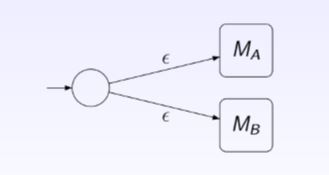
\includegraphics[scale = 0.7]{langunion}}
\caption{Union of two natural languages $M_{A}$ and $M_{B}$}
\label{fig}
\end{figure}
\newpage
\noindent \textcolor{RoyalBlue}{\textbf{Composition of Regular Languages:}} The class of regular languages is closed under $\circ$ (A $\circ$ B)\\
We can construct a NFA by connecting the end states of A and connecting it to the start state of B.  \\\\
\textcolor{RoyalBlue}{\textbf{Kleene Star of Regular Languages:}} The class of regular languages is closed under Kleene star. \\
We can construct a NFA by adding a final state as the start state (for $\epsilon$), and connecting the final state to the original accept state.  \\\\
\noindent \textcolor{RoyalBlue}{\textbf{Regular languages:}} Closed under intersection, complement, difference, and reversal. \\\\
\begin{figure}[h!]
\centerline{ 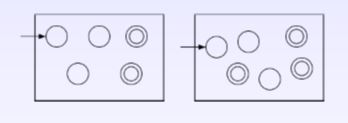
\includegraphics[scale = 0.7]{langcomposition0}}
\caption{Given two languages A and B}
\label{fig}
\vspace{1cm}
\centerline{ 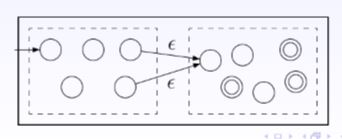
\includegraphics[scale = 0.7]{langcomposition}}
\caption{Creating a NFA of A $\circ$ B}
\label{fig}
\vspace{1cm}
\centerline{ 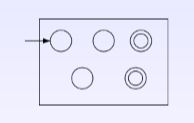
\includegraphics[scale = 0.7]{langkleen0}}
\caption{Given a language A}
\label{fig}
\vspace{1cm}
\centerline{ 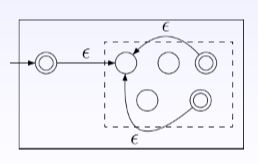
\includegraphics[scale = 0.7]{langkleen}}
\caption{Creating a NFA to recognise $A^{*}$}
\label{fig} 
\end{figure}
\newpage
\noindent \textcolor{RoyalBlue}{\textbf{Minimal DFA:}} Has the smallest possible number of states  \\
\begin{enumerate}
\item Reverse the NFA 
\item Determinize the result 
\item Reverse again 
\item Determinize  \\
\end{enumerate}
Reversing an NFA with an initial state $q_{0}$ and accept states $F \neq \emptyset$: 
\begin{enumerate}
\item If F = \{q\}, then let q be the accept state 
\item Otherwise add a new state q which becomes the only accept state; then, for each state in F, add an $\epsilon$ transition to q. 
\item Reverse every transition in the resulting NFA, making q the initial state and $q_{0}$ the only accept state
\end{enumerate}
\newpage
\section*{Week 8 - Non-Regular Languages \& Context-Free Languages}
\textcolor{RoyalBlue}{\textbf{Regular Expressions:}} The regular expressions over an alphabet $\Sigma = \{a_{1}, ... a_{n}\}$ are given by the grammar:\\
\begin{equation*}
regexp \rightarrow a_{1} \ | \  ...\  | \ a_{n}\  |\  \epsilon \ |\  \emptyset \ |\  regexp \ \cup \ regexp  \ | \ regexp\  regexp\  |\  regexp*
\end{equation*}
\begin{align*}
L(a) &= \{a\} \\ 
L(\epsilon) &= \{\epsilon \} \\ 
L(\emptyset) &= \emptyset \\
L(R_{1} \cup R_{2}) &= L(R_{1}) \cup L(R_{2})\\ 
L(R_{1} R_{2}) &= L(R_{1}) \circ L(R_{2}) \\ 
L(R^{*}) &= L(R)^{*}
\end{align*}
\textcolor{RoyalBlue}{\textbf{Regular Expressions vs Automata:}} L is regular iff L can be described by a regular expression. 
\renewcommand{\labelitemi}{\textperiodcentered}
\begin{itemize}
\item Start by constructing a NFA from the innermost expressions. 
\item Build an NFA with at most one accept state, by using $\epsilon$ transitions from the previous final states to the new final state
\item Label arcs with regular expressions 
\item Repeatedly eliminate states that are neither start nor accept states. 
\end{itemize}
\textcolor{RoyalBlue}{\textbf{Laws for Regular Expressions:}} 
\renewcommand{\labelitemi}{\textperiodcentered}
\begin{align*}
A \cup A &= A \\ 
A \cup B &= B \cup A \\
(A \cup B) \cup C &= A \cup (B \cup C) = A \cup B \cup C \\
(A \  B ) \ C &= A \ (B \ C) = A \ B \ C \\
\emptyset \cup A &= A \cup \emptyset = A  \\
\epsilon \ A &= A \ \epsilon = A \\
\emptyset \ A &= A \ \emptyset = \emptyset \\
(A \cup B) \  C &= A \ C \cup \ B \ C \\
A (B \cup C) &= A \ B \cup A \ C \\
A \ (B \cup C) &= A \ B \cup A \ C \\
(A^{*})^{*} &= A^{*} \\ 
\emptyset_{*} &= \epsilon^{*} = \emptyset \\
(\epsilon \cup A )^{*} &= A^{*} \\
(A \cup B)^{*} &= (A^{*}B^{*})^{*}
\end{align*}
\textcolor{RoyalBlue}{\textbf{Pumping Lemma: }} A standard tool for proving languages are non-regular. \\ 
If A is regular then there is a number p such that for any string $s \in A$ with $|s| \geq p$ s can be written as $s = xyz$  satisfying:
\renewcommand{\labelitemi}{\textperiodcentered}
\begin{itemize}
\item $xy^{i}z \in A$ for all $i \geq 0$
\item $y \neq \epsilon$
\item $|xy| \leq p$ 
\end{itemize}
Where p is the pumping length. \\\\ 
\newpage
\noindent \textcolor{PineGreen}{\textbf{Grammar:}} A grammar is a set of substitution rules or productions.  \\\\
\textcolor{PineGreen}{\textbf{Derivation:}} Using two grammar rules to rewrite a string.  \\\\
\textcolor{PineGreen}{\textbf{Variable:}} `A' is a variable, it can represent other letters. \\\\
\textcolor{PineGreen}{\textbf{Terminal:}} `a', `b', `0', `1' are terminals. They have the same value (cannot be substituted). \\\\
\textcolor{PineGreen}{\textbf{Sentence:}} A string of terminals (cannot substitute anymore) \\\\
\textcolor{PineGreen}{\textbf{Sentential form:}} Intermediate strings that mix variables and terminals during the process of derivation. \\\\
\textcolor{PineGreen}{\textbf{Context-free language (CFL):}} A language which can be generated by some context-free grammar is a context free language.  \\
More formally, it can be represnted as a 4-tuple $(V, \Sigma, R, S)$\\ 
\begin{enumerate}
\item $V$ is a finite set of variables 
\item $\Sigma$ is a finite set of terminals 
\item $R$ is a finite set of rules, each consisting of a variable (the left-hand side) and a string in $(V \cup \Sigma)^{*}$ the right hand side 
\item S is the start variable
\end{enumerate}
The binary relation $\Rightarrow$ on $(V \cup \sigma)^{*}$ is defined as follows: \\ 
Let u,v,w $\in (V \cup \Sigma)^{*}$. Then $uAw \Rightarrow uvw$ iff $A \rightarrow v$ is a rule in R. That is $\Rightarrow$ captures a single derivation step. \\ \\
Let $\overset{*}{\Rightarrow}$ be the \emph{reflexive transitive closure} of $\Rightarrow$. \\
\begin{equation*}
L(G) = \{s \in \Sigma^{*} | S \overset{*}{\Rightarrow} s\}
\end{equation*}
\textcolor{PineGreen}{\textbf{Parse Trees:}} Represents the order from which a sentence is derived. They differ in the order we choose to replace variables. \emph{Leftmost} derviation means we start replacing variables from the left.  \\\\
\textcolor{PineGreen}{\textbf{Ambiguous:}} If a grammar has different parse trees for a sentence. Sometimes the same language can be represented by different grammar, one which is ambiguous and one which may not be ambiguous. \\\\
\newpage 
\section*{Week 9 - Pushdown Automata}
\textcolor{ForestGreen}{\textbf{Pushdown Automaton:}} A finite-state automaton, equipped with a stack. Instead of consuming an input, it can also move the input into a stack and later `pop' it. Based on the input symbol, top stack symbol and current state, the PDA will decide which state to go to next and the operation it will apply to the stack (ie. pop, push or both) \\\\
More formally, a pushdown automaton is a 6-tuple $(Q, \Sigma, \lceil, \delta, q_{0}, F)$
\renewcommand{\labelitemi}{\textperiodcentered}
\begin{itemize}
\item $Q$ is a finite set of states 
\item $\Sigma$ is a finite input alphabet 
\item $\lceil$ is the finite stack alphabet 
\item $\delta: Q \times \Sigma_{\epsilon} \times \lceil_{\epsilon} \rightarrow P(Q \times \lceil_{\epsilon})$ is the transition function 
\item $q_{0} \in Q$ is the start state 
\item $F \subseteq$ Q are the accept states \\
\end{itemize}
Example Transitions: \\\\
$\delta(q_{5}, a, b) = \{(q_{7}, \epsilon)\}$ \\ 
If in state $q_{5}$, if the input is a, and the top of the stack is b, then consume a, pop b and move to state $q_{7}$ \\\\ 
$\delta(q_{5}, \epsilon, b) = \{(q_{6}, a), (q_{7}, b)\}$ \\ 
If the state is $q_{5}$ and the top of the stack is b, then either replace b by a and go to state $q_{6}$ or leave the stack as is and go to state $q_{7}$. Neither of these options consumes an input symbol. \\\\
\textcolor{ForestGreen}{\textbf{Recognisers:}} Every context free language has a PDA which can recognise said language. Every PDA also recognises a context-free language.\\\\
\textcolor{ForestGreen}{\textbf{CFL Properties:}} Closed under union, concatenation, Kleene star, reversal. Not closed under intersection or complement.\\\\
\textcolor{ForestGreen}{\textbf{Deterministic PDA:}} Less powerful than PDAs as it doesn't allow epsilon transitions and doesn't know when to start popping a stack or where the middle is. 
\newpage
\section*{Week 10 - Well-foundness and Turing Machines}
\textcolor{JungleGreen}{\textbf{Partial Functions:}} More commonly used in computer science, as a function may be undefined for some x. \\\\
Notation: $ f:F \hookrightarrow Y$ means that f has a domain that is a subset of X, but f(x) may be undefined for some $x \in X$\\\\
\textcolor{JungleGreen}{\textbf{Total Functions:}} A function that is defined for all inputs of the correct type. (I.e defined for the domain it's given, not necessarily all real numbers)\\\\
\textcolor{JungleGreen}{\textbf{Collatz's problem:}} Deciding whether or not a function is total and will terminate for all n. \\\\
\textcolor{JungleGreen}{\textbf{Termination:}} \\
We can prove termination by looping through a program. 
\begin{enumerate}
\item The measure is a natural number 
\item The measure gets smaller with each loop iteration
\end{enumerate}
The program must terminate for all input, because a natural number cannot be made smaller indefinitely (stops at 0 or 1) \\\\
\textcolor{JungleGreen}{\textbf{Well-founded:}} A binary relation $\prec$ over some set X is well-founded iff there is no infinite sequence of X-elements $x_{1}, x_{2}, x_{3}$ such that
\begin{equation*}
 x_{1} \succ x_{2} \succ x_{3}....
\end{equation*}
Hence (X, $\prec$) is a well-founded structure (will end at some point) \\\\
\textcolor{JungleGreen}{\textbf{Component-Wise Ordering:}} The total of each components contributes to its ordering. Eg. (1,1) and (2,0) would be the same (level/order)\\
\begin{align*}
(x_{1}, x_{2}) \preceq (y_{1}, y_{2}) &\textrm{ iff } x_{1} \leq y_{1} \land x_{2} \leq y_{2} \\
p \preceq q &\textrm{ iff } p \preceq q \land p \neq q
\end{align*}
\textcolor{JungleGreen}{Hasse Diagram:} Can be used for a component wise ordering of  $\mathbb{N} \times \mathbb{N}$ (i.e tuples)\\
Values increase as you travel up edges \\\\
\textcolor{JungleGreen}{\textbf{Lexographical ordering:}} Similar to the alphabet, the earlier positions take precence when ordering. Eg. (1,100) $\preceq$ (100,1) \\\\
\textcolor{JungleGreen}{\textbf{Well founded orderings on tuples:}}
\renewcommand{\labelitemi}{\textperiodcentered}
\begin{itemize}
\item \textbf{Theorem:} If $\prec$ is well-founded, then so is its component wise extension to tuples. 
\item \textbf{Theorem:} If $\prec$ is well-founded then so is its lexicographic extension to tuples. 
\item If all of the elements and the ordering function is well-founded, then any combination of tuples with said element and ordering can be grouped component wise or lexicographically. 
\end{itemize}
\textcolor{JungleGreen}{\textbf{Well-founded Induction:}} An induction principle that goes with well-founded relations. Given that a structure is well-founded (X, $\prec$), we can prove a statement ``for all x $\in$ X, S(x)'' by assuming that S(x') holds for all $x' \prec x$, and use that to establish S(x). \\\\
\newpage
\noindent \textcolor{JungleGreen}{\textbf{Undeciable Problems:}} Problems that have no algorithm for solving it. \\\\
\textcolor{JungleGreen}{\textbf{Turing Machine:}} Has an unbounded tape through which it takes its input and performs computations. It is able to both write and read to the tape, and move left and right over the tape. The machine's accept and reject states are irrespective of the tape head. \\
Formally: \\ 
A Turing Machine is a 7-tuple $M = (Q, \Sigma, \lceil, \delta, q_{0}, q_{a}, q_{r})$ where: 
\renewcommand{\labelitemi}{\textperiodcentered}
\begin{itemize}
\item $Q$ is a finite set of states 
\item $\lceil$ is a finite tape alphabet, including the blank character \textvisiblespace
\item $\Sigma \subseteq \lceil \  \backslash \{ \textvisiblespace \}$ is the input alphabet (Sigma is a subset of the tape alphabet without the blank character)
\item $\delta: Q \times \lceil \rightarrow Q \times \lceil \times \{L,R\}$ is the transition function 
\item $q_{0}$ is the initial state 
\item $q_{a}$ is the accept state
\item $q_{r} (\neq q_{a})$ is the reject state
\end{itemize}
Transition function $\delta(q_{i}, x) = (q_{j}, y, d)$ depends on two things 
\begin{enumerate}
\item The current state $q_{i}$
\item The current symbol x under the tape head 
\end{enumerate}
It consists of three actions 
\begin{enumerate}
\item change state to $q_{j}$
\item overwrite tape symbol x by y 
\item move the tape head in the direction of d
\end{enumerate}
\textcolor{JungleGreen}{\textbf{Computations:}} \\\\
For all $q_{i}, q_{j} \in Q$, $a,b,c \in \lceil$ and $u,v \in \lceil^{*}$ we have\\ 
\begin{align*}
uq_{i}bc \Rightarrow ucq_{i}v \ &\textrm{if } \delta(q_{i}, b) = (q_{j}, c, R) \\
q_{i}bv \Rightarrow q_{j}cv \ &\textrm{if } \delta(q_{i}, b) = (q_{j}, c, L) \\
uaq_{i}bv \Rightarrow uq_{j}acv \ &\textrm{if } \delta(q_{i}, b) = (q_{i}, c, L)
\end{align*}
The start configuration of M on input w is $q_{0}w$ \\
M accepts w iff there is a sequence of configurations $C_{1}, C_{2}... C_{k}$ such that 
\begin{enumerate}
\item $C_{1}$ is the start configuration $q_{0}w$ \\
It is a valid start state
\item $C_{i} \Rightarrow C_{i+1}$ for all $i \in \{1...k-1\}$\\
Every configuration has a valid transition
\item The state of $C_{k}$ is $q_{a}$ \\
The final configuration ends in an accept state
\end{enumerate}
\textcolor{JungleGreen}{\textbf{Turing recognisable:}} A language A is Turing reconisable (or recursively enumerable) iff A = L(M) for some TUring machine M. There exists a Turing Machine that recognises it.\\\\
\textcolor{JungleGreen}{\textbf{Turing behaviors:}} A Turing machine M can accept an input w, can reject w or fail to halt on w. \\\\
\textcolor{JungleGreen}{\textbf{Turing decidable:}} If a Turing machine M halts on all input of language A, then M decides A. \\\\
\newpage 
\section*{Week 11 - Decidable and Undecidable Languages}
\textcolor{Peach}{\textbf{Multitape Machines:}} A multitape Turing machine has k tapes. It takes input on tape 1 and the other tapes are blank. It can write and move to other tapes, and specifies through the transitions how k tape heads behave when the machine is in state $q_{i}$ and reading some alphabet. \\
\begin{equation*}
\textrm{Transition Function: } \delta: Q \times \lceil^{k} \rightarrow Q \times \lceil^{k} \times \{L,R\}^{k}
\end{equation*}
eg. 
\begin{equation*}
\delta (q_{i}, a_{1}, ... a_{k}) = (q_{j}, (b_{1}, ... b_{k})(d_{1}...d_{k}))
\end{equation*}
\textcolor{Peach}{\textbf{Theorem:}} A language is Turing recognisable iff some multitape Turing Machine recognises it. We can simulate a multitape machine M by using a standing Turing machine S. Instead of using seperators $\#$, we can just put new string segments into a new tape.  \\\\
\textcolor{Peach}{\textbf{Nondeterministic Turing Machines:}} If some computation leads to an accept state, then the machine accepts the input. A nondeterministic Turing machine has a transition function of type: \\
\begin{equation*}
\delta: Q \times \lceil \rightarrow P(Q \times \lceil \times \{L,R\})
\end{equation*}
\textcolor{Peach}{\textbf{Theorem:}} A language is Turing recognisable iff some nondeterministic Turing machine recognises it. I.e every nondeterministic Turing machine N can be simulated by a deterministic Turing machine D. \\\\
\textcolor{Peach}{\textbf{Enumerator:}} A Turing machine built to generate all strings in a language L. For an enumerator to enumerate a language L, for each string in L, it must eventually print said string. \\\\
\textcolor{Peach}{\textbf{Theorem:}} L is Turing recognisable iff some enumerator enumerates L. \\
Proof: \\
\begin{enumerate}
\item Let E be an enumerator for L
\item Let w be the input
\item Simulate E. For each string s output by E, if s = w then accept. 
\end{enumerate}
Alternatively: \\ 
\begin{enumerate}
\item Let i = 1, and M be a Turing machine that recognises L. E produces strings `$s_{i}$'. 
\item Simulate M for i steps on each of $s_{1},...s_{i}$
\item For each accepting computation, print that s 
\item Increment i and go to step 2 
\end{enumerate}
\textcolor{Peach}{\textbf{Acceptance Problem:}} For DFAs, the acceptance problem is if a DFA D accepts input w. \\\\
\textcolor{Peach}{\textbf{Theorem:}} $A_{DFA}$ is a decidable language\\
Proof: \\ 
We can use a Turing Machine M to simulate a DFA D. For example, a turing machine M can have a tape with the input: \\ 
Q(states) \#\# $\Sigma$(alphabet) \#\# $\delta$(transitions) \#\# $q_{0}$(initial state) \#\# $F$(final states) \#\# w(string) \$ \\ \\
eg.
\begin{center}
\#1...n \#\#ab..z\#\#1a2\#...\# nbn\#\#1\#\#3 7 \#\# baa...\$
\end{center}
M first checks if the first five components represent a valid DFA, and if it doesn't it will reject it. Then M simulates the moves of D, keeping track of D's state and the current position in w by writing the details on the tape after \$. When the last symbol w has been processed, M accepts if D is in a state in F, otherwise rejects. \\\\
\textcolor{Peach}{\textbf{Theorem:}}$A_{NFA}$ is decidable. We can do this by using a halting Turing Machine to translate an NFA to a DFA, and then use the previous theorem to run it. \\\\
\textcolor{Peach}{\textbf{Theorem:}} $E_{DFA}$ is decidable (Determining if a DFA is empty)\\
\begin{center}
$E_{DFA} = \{<D> | D \textrm{is a DFA and L(D)} = \emptyset\}$
\end{center}
Proof:
\begin{enumerate}
\item Design a Turing machine that takes $<$D$>$ = $(Q, \Sigma, \delta, q_{0}, F)$ as input and performs a reachability analysis: 
\item Set reachable = \{$q_{0}$\}, D's start state 
\item Set new = \{$q | \delta(m,x) = q$, m $\in$ reachable\} \ reachable 
\item If new $\neq \emptyset$, set reachable = reachable $\cup$ new and go to step 3 
\item If reachable $\cap$ F $= \emptyset$ accept, otherwise reject (If we can't reach the accept state, then accept the DFA)
\end{enumerate}
\textcolor{Peach}{\textbf{Theorem: }} $EQ_{DFA}$ DFA equivalence is decidable\\
\begin{center}
$EQ_{DFA}= \{<A,B> | \textrm{A and B are DFAs and L(A) = L(B)}\}$
\end{center}
Proof: \\ 
We can construct DFAs using intersection, union and complement which are mechanistic and finite. Therefore a Turing Machine M can perform those actions. From a DFA A and B, M can produce a DFA C to recognise \\
\begin{center}
L(C) = (L(A) $\cap$ L(B$)^{c}$) $\cup$ (L(A$)^{c}$ $\cap$ L(B)) \\ 
L(C) = $\emptyset$ iff L(A) = L(B)
\end{center}
We can use the emptiness checker on C. \\\\
\textcolor{Peach}{\textbf{Theorem:}} $A_{CFG}$ Generation by CFGs is Decidable. \\
\begin{center}
$A_{CFG} = \{<G, w> | \textrm{G is a CFG that generates w}\}$
\end{center}
Proof: \\ 
We can reqrite any CFG to Chomsky Normal Form. Each production takes one of two forms: 
\begin{center}
A $\rightarrow$ B C    or   A $\rightarrow$ a  and S $\rightarrow$  $\epsilon$ (start) 
\end{center}
For every grammar in Chomsky Normal Form form, if string w can be derived, then the derivation has exactly 2(w) - 1 steps. It is similar to a binary tree. To decide $A_{CFG}$ we can simply try out all possible derivations of that length, in finite time and see if one generates w. \\\\
\newpage
\noindent \textcolor{Peach}{\textbf{Theorem:}} $E_{CFG}$ CFG Emptiness is Decidable \\
\begin{center}
$E_{CFG} = {<G> | G \textrm{is a CFG and L(G)} = \emptyset}$
\end{center}
Proof: \\ 
We can design a Turing Machine which takes $<G> = (V, \Sigma, R, S)$ as input, and performs a `producer' analysis 
\begin{enumerate}
\item Set producers = $\Sigma$, all of G's terminals
\item Set new = (\{$A | A \rightarrow U_{1} ... U_{n} \in R$\} and \{$A | \{U_{1}...U_{n}\} \subseteq \textrm{producers}$\}) $\backslash$ producers 
\item If new $\neq \emptyset$ producers = producers $\cup$ new and go to step 2 
\item If S $\in$ producers, reject otherwise accept
\end{enumerate}
\textcolor{Peach}{\textbf{Theorem:}} Every CFL is decidable. \\\\
Proof: We can specialise a decider S. Let $G_{0}$ be a CFG for $L_{0}$. The decider for $L_{0}$ simply takes input w and runs S on $<G_{0}, w>$
\newpage
\noindent \textcolor{Orange}{\textbf{Undecidable problems:}} If a turing machine accepts a given string, then the turing machine may fail to halt.   \\\\
\textcolor{Orange}{\textbf{Theorem:}} $A_{TM}$ Turing machine acceptance is undecidable. \\
\begin{center}
$A_{TM}$ = \{$<M,w> | $ M is a TM and M accepts w\}
\end{center}
Proof: \\ 
Assume (for contradiction) that $A_{TM}$ is decided by a TM H, where H accepts if M accepts w, and rejects if M rejects w. \\ 
Using H we can construct a Turing machine D which decides whether a given machine M fails to accept its own encoding $<M>$: 
\begin{enumerate}
\item Input is $<M>$, where M is some Turing machine. 
\item Run H on $<M, <M>>$
\item If H accepts, reject. If H rejects, accepts. 
\end{enumerate}
Step 3 produces a contradiction, as we're saying if M accepts, then reject M. Therefore no such Turing Machine can evaluate it's own encoding. \\\\
\textcolor{Orange}{\textbf{Bijections and Enumeration:}} A bijection in $\mathbb{N} \rightarrow X$ gives us an enumeration of the set X. \\\\
\textcolor{Orange}{\textbf{Sizes of Infinite Sets:}}
\renewcommand{\labelitemi}{\textperiodcentered}
\begin{itemize}
\item card(X) $\leq$ card(Y) iff there is a total, injective f: X $\rightarrow$ Y 
\item card(X) = card(Y) iff card(X) $\leq$ card(Y) and card(Y) $\leq$ card(X)
\end{itemize}
\textcolor{Orange}{\textbf{Countable:}} X is countable iff card(X) $\leq$ card($\mathbb{N}$) \\\\
\textcolor{Orange}{\textbf{Countably Infinite:}} X is countably infinite iff card(X) = card($\mathbb{N}$) \\\\
\textcolor{Orange}{\textbf{Uncountable:}}$\mathbb{N} \rightarrow \mathbb{N}$ is uncountable, and can be shown through diagonalization\\\\
\textcolor{Orange}{\textbf{Theorem:}} There is no bijection h: $\mathbb{N} \rightarrow (\mathbb{Z} \rightarrow \mathbb{Z})$ \\\\
Proof: \\ 
Assume h exists. Then h(0), h(1) ... h(n) ... contains every function in $\mathbb{Z} \rightarrow \mathbb{Z}$ without duplicates. \\ 
Now constructing f: $\mathbb{Z}\rightarrow \mathbb{Z}$ as f(n) = h(n)(n) + 1. \\ 
Then f $\neq$ h(n) for all n, so we have a contradiction. 
\newpage 
\section*{Week 12 - Reducibility}
\textcolor{Orange}{\textbf{Theorem:}} A language L is decidable iff both L and the complement of L is Turing recognisable. If L is decidable, then L and $l^{c}$ are recognisable.  \\\\
\textcolor{Orange}{\textbf{Theorem:}} $E_{TM}$, Emptiness of a Turing Machine is Undecidable.
\begin{equation*}
E_{TM} = \{<M> | \ \textrm{M is a TM and L(M)} = \emptyset \}
\end{equation*}
Proof: \\ 
$A_{TM}$ is reducable to $E_{TM}$. Given $<M,w>$, a Turing machine can modify the encoding of M so as to turn M into M' which recognises L(M) $\cap$ \{w\}. Running the machine then putting the output into the modified machine, we receive a contradiction. \\\\
\textcolor{Orange}{\textbf{Rice's Theorem:}} Every interesting semantic Turing machine property is undecidable. A property is interesting iff it holds for some TMs but not others. It is semantic iff it holds for all Turing machines that accept the same language. \\\\
\textcolor{Orange}{\textbf{}} \\\\
\textcolor{Orange}{\textbf{}} \\\\
\end{document} 
